% Options for packages loaded elsewhere
\PassOptionsToPackage{unicode}{hyperref}
\PassOptionsToPackage{hyphens}{url}
\documentclass[
  10pt,
]{article}
\usepackage{xcolor}
\usepackage[margin=20mm]{geometry}
\usepackage{amsmath,amssymb}
\setcounter{secnumdepth}{-\maxdimen} % remove section numbering
\usepackage{iftex}
\ifPDFTeX
  \usepackage[T1]{fontenc}
  \usepackage[utf8]{inputenc}
  \usepackage{textcomp} % provide euro and other symbols
\else % if luatex or xetex
  \usepackage{unicode-math} % this also loads fontspec
  \defaultfontfeatures{Scale=MatchLowercase}
  \defaultfontfeatures[\rmfamily]{Ligatures=TeX,Scale=1}
\fi
\usepackage{lmodern}
\ifPDFTeX\else
  % xetex/luatex font selection
\fi
% Use upquote if available, for straight quotes in verbatim environments
\IfFileExists{upquote.sty}{\usepackage{upquote}}{}
\IfFileExists{microtype.sty}{% use microtype if available
  \usepackage[]{microtype}
  \UseMicrotypeSet[protrusion]{basicmath} % disable protrusion for tt fonts
}{}
\makeatletter
\@ifundefined{KOMAClassName}{% if non-KOMA class
  \IfFileExists{parskip.sty}{%
    \usepackage{parskip}
  }{% else
    \setlength{\parindent}{0pt}
    \setlength{\parskip}{6pt plus 2pt minus 1pt}}
}{% if KOMA class
  \KOMAoptions{parskip=half}}
\makeatother
\usepackage{graphicx}
\makeatletter
\newsavebox\pandoc@box
\newcommand*\pandocbounded[1]{% scales image to fit in text height/width
  \sbox\pandoc@box{#1}%
  \Gscale@div\@tempa{\textheight}{\dimexpr\ht\pandoc@box+\dp\pandoc@box\relax}%
  \Gscale@div\@tempb{\linewidth}{\wd\pandoc@box}%
  \ifdim\@tempb\p@<\@tempa\p@\let\@tempa\@tempb\fi% select the smaller of both
  \ifdim\@tempa\p@<\p@\scalebox{\@tempa}{\usebox\pandoc@box}%
  \else\usebox{\pandoc@box}%
  \fi%
}
% Set default figure placement to htbp
\def\fps@figure{htbp}
\makeatother
\setlength{\emergencystretch}{3em} % prevent overfull lines
\providecommand{\tightlist}{%
  \setlength{\itemsep}{0pt}\setlength{\parskip}{0pt}}
\usepackage{fontspec}
\usepackage{xeCJK}
\setCJKmainfont{Microsoft YaHei}
\setmainfont{TeX Gyre Termes}
\usepackage{tikz,pgfplots}
\pgfplotsset{compat=1.18}
\usepackage{float}
\let\origfigure\figure
\let\endorigfigure\endfigure
\renewenvironment{figure}[1][]{\origfigure[H]}{\endorigfigure}
\usepackage{graphicx}
\setlength{\emergencystretch}{3em}
\usepackage{fancyhdr}
\pagestyle{fancy}
\fancyhf{}
\fancyfoot[C]{\thepage}
\renewcommand{\headrulewidth}{0pt}
\usepackage{bookmark}
\IfFileExists{xurl.sty}{\usepackage{xurl}}{} % add URL line breaks if available
\urlstyle{same}
\hypersetup{
  hidelinks,
  pdfcreator={LaTeX via pandoc}}

\author{}
\date{}

\begin{document}

\section{中文导读：同一颗核，为什么换个位置就可能找到}\label{ux4e2dux6587ux5bfcux8bfbux540cux4e00ux9897ux6838ux4e3aux4ec0ux4e48ux6362ux4e2aux4f4dux7f6eux5c31ux53efux80fdux627eux5230}

本轮先后检验了三个问题：把预测点移动到更准确的位置是否有效；平均多个平移图像的分数是否有效；平移训练模型是否因为分数偏低而被阈值排除。现在又用保存的预测点，把每颗漏检核的情况分开。

八个模型均完成了最新实验，一次保存故障已经补齐。最值得记住的区别是：全层检测器的漏检多受对齐影响，平移训练检测器则有更多核已经定位、分数却低于原阈值。

\newpage

\section{训练图像接近99\%，为什么仍会漏检}\label{ux8badux7ec3ux56feux50cfux63a5ux8fd199ux4e3aux4ec0ux4e48ux4ecdux4f1aux6f0fux68c0}

编码器把图像分成16像素的小块。训练时几乎精确找到的核，换一种与小块网格的对齐方式后，检出率降到约70\%。同一张图像、同一颗核，平移几个像素就足以改变预测。

这也是位置读出实验和十六种对齐实验共同给出的线索。移动预测点新增的匹配与丢失的匹配相当；直接平均不同位置的窄分数峰又把峰值压低。后续因此改为汇总点的位置，并独立检查分数阈值。

\begin{center}
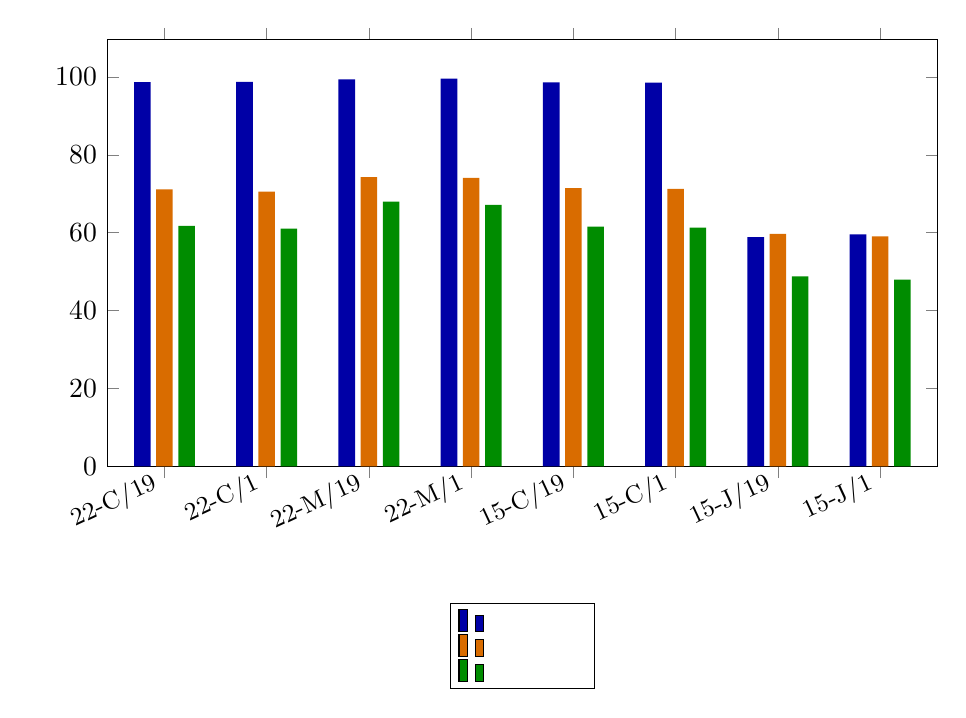
\begin{tikzpicture}
\begin{axis}[width=\linewidth,height=7cm,ymin=0,xtick={0,1,2,3,4,5,6,7},xticklabels={22-C/19,22-C/1,22-M/19,22-M/1,15-C/19,15-C/1,15-J/19,15-J/1},x tick label style={font=\small,rotate=25,anchor=east},ylabel={匹配率（百分比）},legend style={at={(0.5,-0.32)},anchor=north,legend columns=1,font=\small},enlarge x limits=0.08,ybar,bar width=6pt]
\addplot[fill=blue!65!black,draw=none] coordinates {(0,98.654846) (1,98.715989) (2,99.388566) (3,99.602568) (4,98.593702) (5,98.563131) (6,58.850504) (7,59.584225)};
\addplot[fill=orange!85!black,draw=none] coordinates {(0,71.150515) (1,70.537043) (2,74.285132) (3,74.103740) (4,71.478651) (5,71.282992) (6,59.702436) (7,59.082849)};
\addplot[fill=green!55!black,draw=none] coordinates {(0,61.777398) (1,61.091151) (2,67.968824) (3,67.191332) (4,61.573044) (5,61.304059) (6,48.817603) (7,47.957418)};
\legend{训练图像原对齐,训练图像其余十五种对齐,开发评估图像其余十五种对齐}
\end{axis}
\end{tikzpicture}
\end{center}

蓝、橙、绿柱依次比较训练原对齐、训练其他对齐、开发评估其他对齐；后缀为种子。

\newpage

\section{平移训练的模型，为什么降低阈值后找回很多核}\label{ux5e73ux79fbux8badux7ec3ux7684ux6a21ux578bux4e3aux4ec0ux4e48ux964dux4f4eux9608ux503cux540eux627eux56deux5f88ux591aux6838}

平移训练模型在阈值0.5下只找到约38\%的标注核，但两个种子在训练图像上都选出了0.2。保持这些选择，在开发评估图像上找到约69\%---70\%；内部死亡核从44个增加到101、99个。

预测位置没有重新训练，变化来自解码接纳了较低分数的点。与此同时，预测点精度从约86\%降到约66\%。这说明下一步要解决的是如何保留这些核并抑制额外点。

位置一致性汇总保留的点较少，精度约81\%，检出率约52\%---53\%；它仍只汇总分数0.5以上的点。低分数接纳与多对齐位置支持可以在新的、训练侧固定的设计中一起检验。

\newpage

\section{一张结肠组织图像里的三个具体例子}\label{ux4e00ux5f20ux7ed3ux80a0ux7ec4ux7ec7ux56feux50cfux91ccux7684ux4e09ux4e2aux5177ux4f53ux4f8bux5b50}

图中黄色7号核的标注中心为(141,65)，模型原分数0.486，刚好被0.5排除。降至训练侧选出的0.2后能找到；多对齐汇总也找到它，预测点距标注1.90像素。

\begin{figure}
\centering
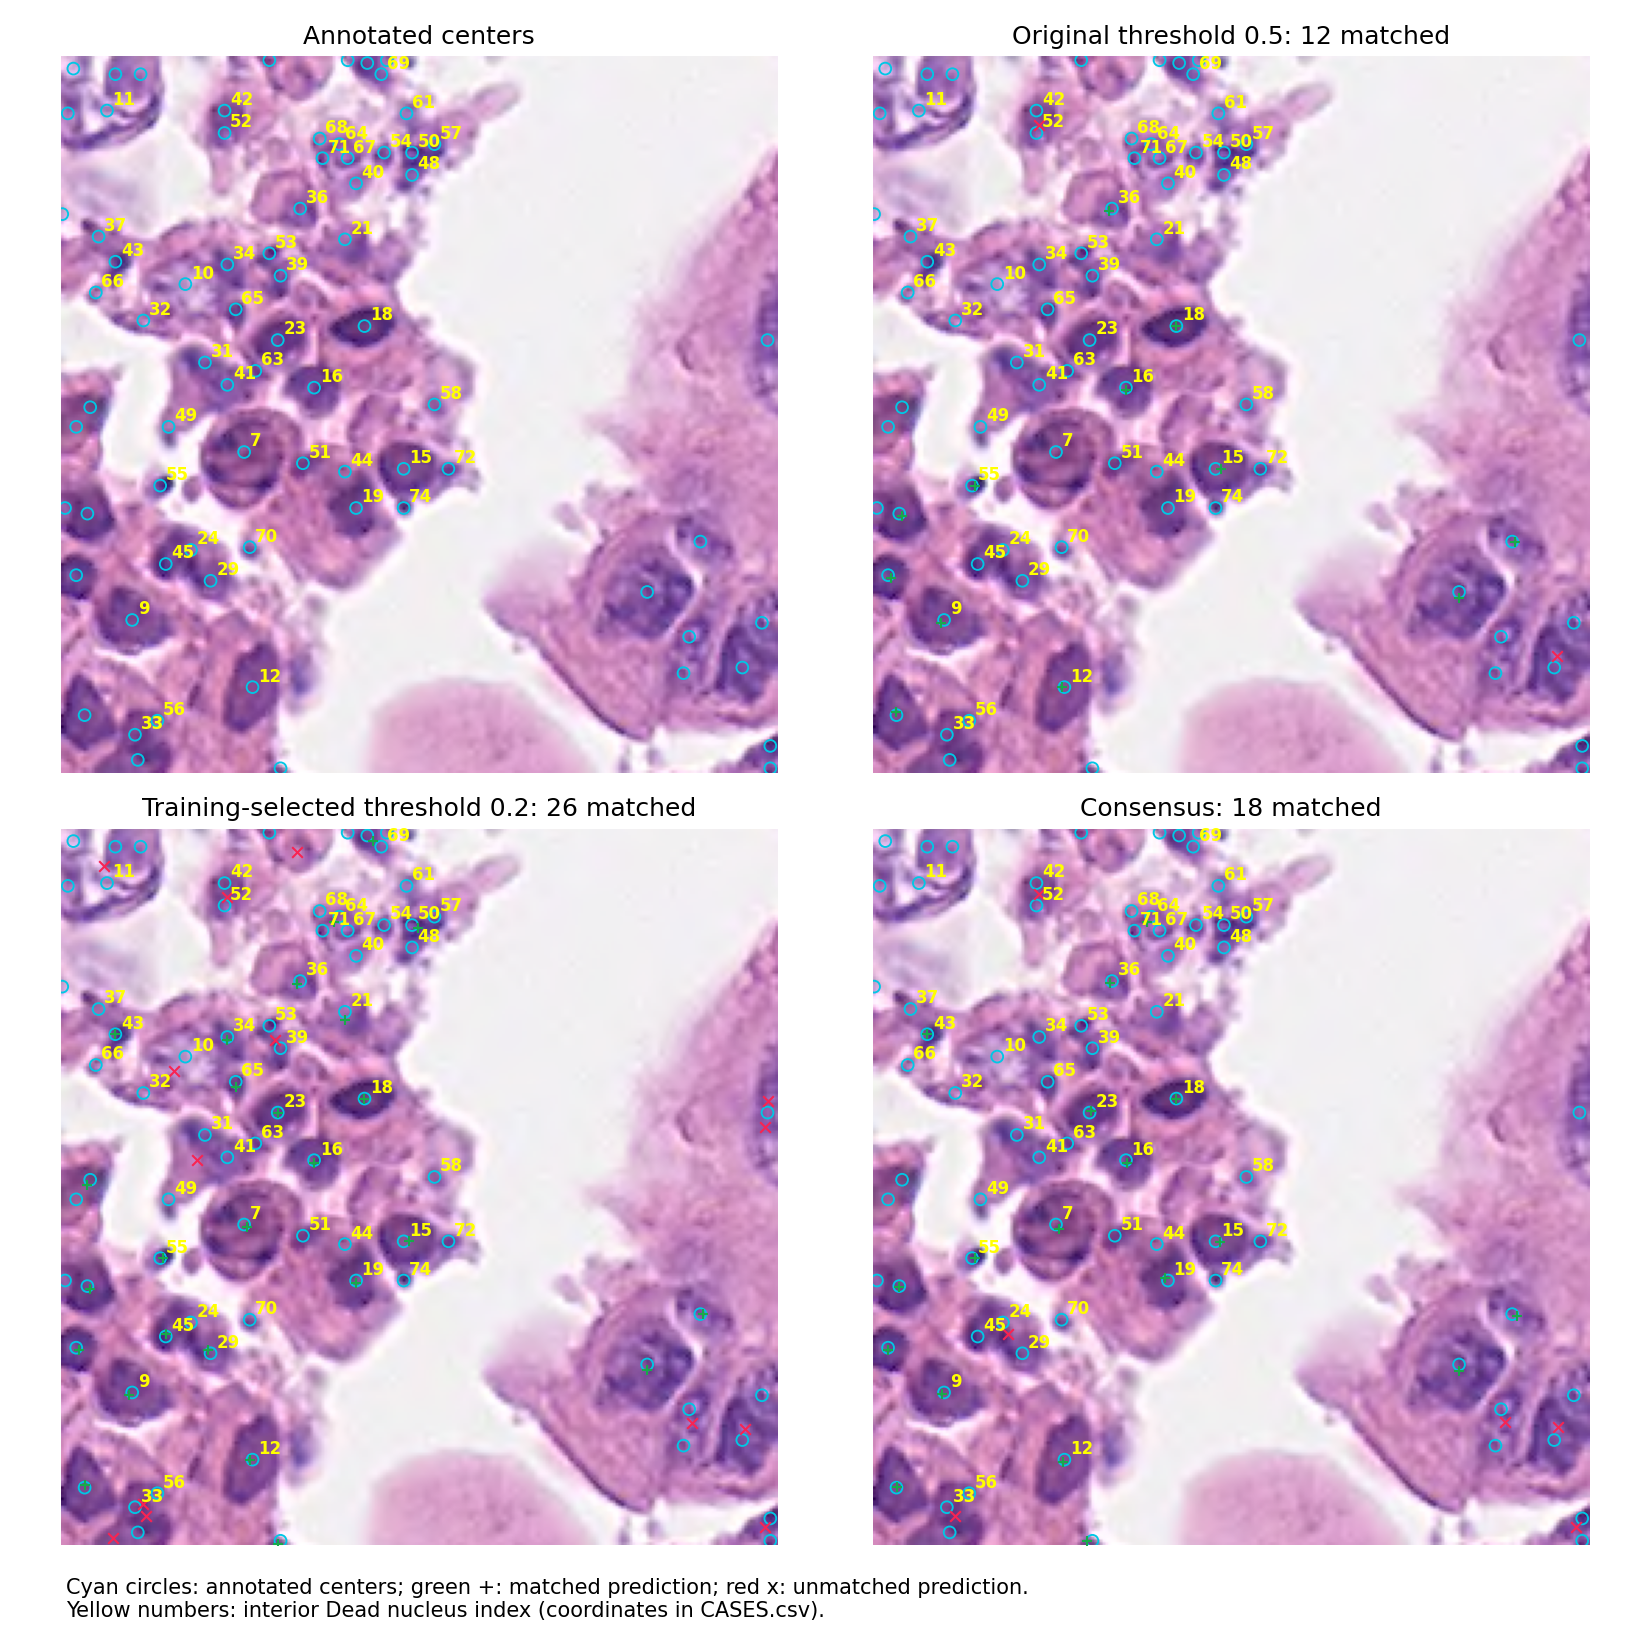
\includegraphics[width=0.9\linewidth,height=\textheight,keepaspectratio,alt={结肠组织图像1482：原解码、选定阈值与位置汇总。}]{assets/P15_J_s19_development_1482.png}
\caption{结肠组织图像1482：原解码、选定阈值与位置汇总。}
\end{figure}

51号核面积67像素，两个检测器在所有对齐、0.1记录下限下都没有三像素内匹配点。附近55号核更小，只有57像素，平移训练模型却找到它。实际图像与坐标告诉我们：小核确实困难，但不能只用面积解释每一次漏检。

\newpage

\section{剩下的核，需要改进哪一个环节}\label{ux5269ux4e0bux7684ux6838ux9700ux8981ux6539ux8fdbux54eaux4e00ux4e2aux73afux8282}

新诊断将每颗核依次归为原来找到、换对齐找到、接纳低分数后找到、近邻分配竞争、所有对齐下仍无三像素内已记录点。下面仅统计离边缘足够远的7014个核。

全层种子19原来漏掉4271个核，其中2476个换对齐可找到，401个只在低分数下找到。平移训练种子19原来漏掉7479个核，其中2104个换对齐可找到，4141个需要低分数点。两类模型的主要困难不同。

\begin{center}
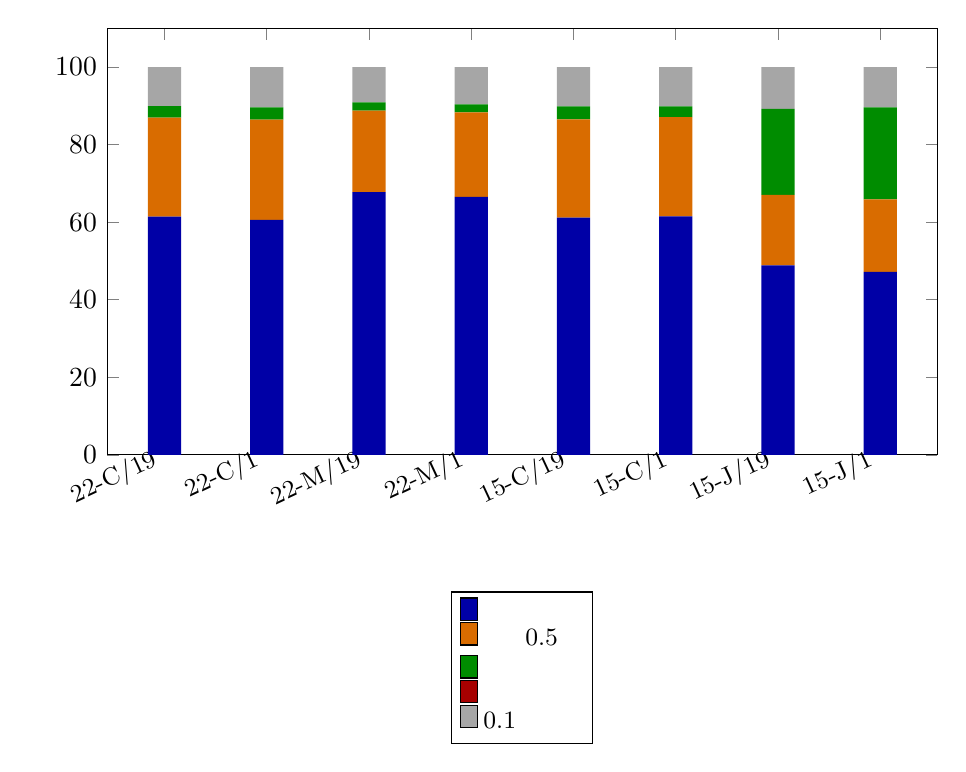
\begin{tikzpicture}
\begin{axis}[width=\linewidth,height=7cm,ymin=0,xtick={0,1,2,3,4,5,6,7},xticklabels={22-C/19,22-C/1,22-M/19,22-M/1,15-C/19,15-C/1,15-J/19,15-J/1},x tick label style={font=\small,rotate=25,anchor=east},ylabel={中心区域标注核（百分比）},legend style={at={(0.5,-0.32)},anchor=north,legend columns=1,font=\small},enlarge x limits=0.08,ybar stacked,bar width=12pt]
\addplot[fill=blue!65!black,draw=none] coordinates {(0,61.448532) (1,60.564585) (2,67.721699) (3,66.524095) (4,61.191902) (5,61.505560) (6,48.873681) (7,47.191332)};
\addplot[fill=orange!85!black,draw=none] coordinates {(0,25.506131) (1,25.862561) (2,21.043627) (3,21.799259) (4,25.320787) (5,25.591674) (6,18.149415) (7,18.676932)};
\addplot[fill=green!55!black,draw=none] coordinates {(0,2.965498) (1,3.136584) (2,2.138580) (3,2.024522) (4,3.321928) (5,2.765897) (6,22.212717) (7,23.709723)};
\addplot[fill=red!65!black,draw=none] coordinates {(0,0.000000) (1,0.000000) (2,0.000000) (3,0.000000) (4,0.000000) (5,0.000000) (6,0.000000) (7,0.000000)};
\addplot[fill=gray!70,draw=none] coordinates {(0,10.079840) (1,10.436270) (2,9.096094) (3,9.652124) (4,10.165384) (5,10.136869) (6,10.764186) (7,10.422013)};
\legend{原对齐匹配,其他对齐在0.5匹配,只在较低分数下匹配,近邻分配竞争,0.1下无三像素内预测点}
\end{axis}
\end{tikzpicture}
\end{center}

五类互斥结局；统计利用标注核检查点是否可用，分数低于0.1的点没有保存。
下一步应在训练侧独立校准低分数点，并检验位置支持能否减少额外点。训练与开发评估角色、两种子与原判定条件继续保留；本阶段结论来自核中心检测。完整报告另有英文版、详细中文版、坐标表与源码。

\end{document}
